\documentclass{article}
\usepackage[utf8]{inputenc}
\usepackage{amsmath}
\usepackage{amssymb}
\usepackage{amssymb}
\usepackage{upgreek}
\usepackage[colorlinks = true, linkcolor = black, urlcolor  = blue]{hyperref}

\usepackage[margin=1.5in]{geometry}
\usepackage{relsize}
\usepackage{color}
\usepackage{graphicx}
\usepackage{subcaption}
\usepackage{algorithm}
\usepackage[noend]{algpseudocode}

\title{Distributed GPU Acceleration for miniFE} 
\author{Ryan Greenblatt}
\date{May 2019}

\begin{document}

\setlength\parindent{0pt}

\renewcommand{\thesubsection}{\alph{subsection}}

\maketitle

\section{Background}

miniFE provides an example application for distributed and threaded CPU finite
element simulations\footnote{The most recent version on Github has CUDA
support, but the variant I worked with had no CUDA support}. Outside of data
setup, miniFE uses the conjugate gradient method for solving a sparse linear
system. While the data setup and initialization could be further parallelized
and some parts could be effectively moved to the GPU, focus was placed on
porting the conjugate gradient method to run distributed on GPUs. The algorithm
for the method is detailed below. The kernels involved in applying the method
to a sparse system include the dot product, sparse matrix dense vector
multiplication (SpMV), and WAXPBY (element wise multiplication). As such, this
algorithm is well suited to GPU acceleration, but is certainly going to
be memory bandwidth limited.

\begin{algorithm}
  % \caption{Conjugate Gradient Method}
  \begin{algorithmic}[1]
    \Procedure{Conjugate Gradient Method}{$A, x, b, \epsilon$}
    \State $r_0 \gets b - A x$
    \State $r_1 \gets r_0$
    \State $p \gets r_0$
    \State $i \gets 1$
  \While{$\Vert r_i \Vert_2 > \epsilon \text{ and } i \leq \text{max\_iter}}$}
    \State $p \gets r_i + \frac{\Vert r_i \Vert_2^2}{\Vert r_{i-1} \Vert_2^2} p$
    \State $\alpha \gets \frac{\Vert r_i \Vert_2^2}{\langle A p,  p\rangle}$
    \State $x \gets x + \alpha p$
    \State $r_{i+1} \gets r_i + \alpha A p$
    \State $i \gets i + 1$
    \EndWhile
    \EndProcedure
  \end{algorithmic}
\end{algorithm}

\section{Approach}

While the ELLPACK data format is hypothetically implemented in miniFE, the
original code failed to compile when using that format. As such, the CRS format
was used exclusively. OpenMP is used extensively for CPU threading in the
original code. Because of this, it would have been desirable to use the clang
compiler's support for generating PTX instructions from OpenMP directives.
However, support is relatively new and a known linker bug with no documented
solutions made this challenging, so this approach was not used.  \\

The cuSPARSE and cuBlas libraries were used for dot products and SpMV as they
have highly optimized implementations for these simple operations. \\

The existing code makes heavy use of STL vectors, so a custom 
allocator was used to allocate the vector array as CUDA managed memory.
Managed memory is advantageous for improving interactions with MPI
and making incremental implementation easier. \\

Due to a lack of access to systems with GPU interconnect\footnote{I didn't want
to spend a lot of money on cloud computing}, I used generic MPI message
passing through the CPU. \\

I have modified miniFE so that the original types are no longer configurable,
only int ordinals are used. This was done because a fixed ordinal type is 
needed for cuSPARSE and cuBlas. The scalar type is still configurable and
I tested single and double precision. \\

Code is attached in the email. I have included a CMakeLists.txt file which can
be used to compile the code on the CCV. The \verb cuda/10.0.130 module and some
MPI module must be loaded. Note that gencode is specified to be
``arch=compute\_70,code=sm\_70" which may cause issues on older GPUs. \\


The original miniFE code had a bug that would cause occasional segmentation
faults when running multiple processes and several incomplete and untested
features which weren't clearly labeled as such. In general, the code felt
unfinished. I have tried to polish things somewhat and remove 
partially implemented features. \\

\section{Results}

\begin{figure}[H] 
  \centering
  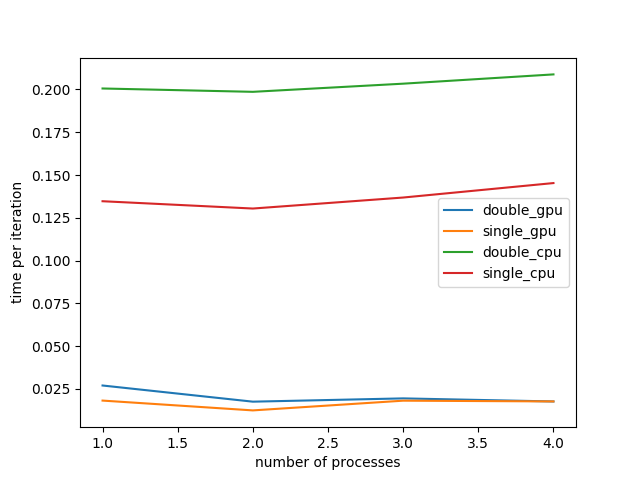
\includegraphics[width=0.8\linewidth]{../gpu_cpu.png}
  \caption{GPU and CPU iteration timings for various numbers of processes and
  different data types. Note that the number of process also corresponds to the 
  number of GPUs used for the GPU computations.}
\end{figure}

Because of the 2 GPU limit I have on the CCV, testing was conducted on a system
with 4 2080 Tis (using a peer to peer cloud provider). CPU only testing was
done with 16 threads. Access to more GPUs would have been ideal to better understand
scaling, but options are limited without substantial spending.  Note that the
setup and initialization take the vast majority of the time when using a GPU on
any problem size which I could feasibly test. This time isn't included in the
results. I tested with all dimensions equal (a cube) and I tested single and
double precision.  Single and double precision appeared to have similar
residuals in this case. \\

\begin{figure}[H] 
  \centering
  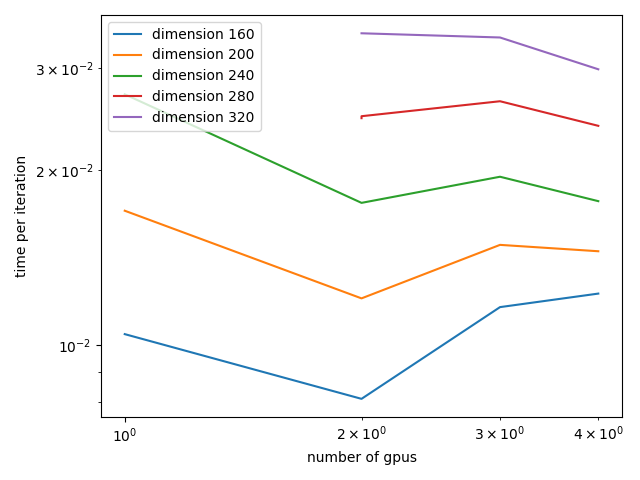
\includegraphics[width=0.8\linewidth]{../strong_scaling.png}
  \caption{Log-log strong scaling plot for various dimensions with double 
    precision.  Not all dimensions could be successfully run with 1 GPU.}
\end{figure}


The GPU implementation is almost an order of magnitude faster than the CPU
implementation. Adding an additional GPU scales the speed of the computation by
almost 2, but further additional GPUs actually resulted in small reductions in
speed. However, memory is likely to often be limited, so more than 2 GPUs may
be needed for larger problem sizes. Because managed memory is used, when memory
runs out on the GPU(s), the computation continues but is greatly slowed. \\

\begin{figure}[H] 
  \centering
  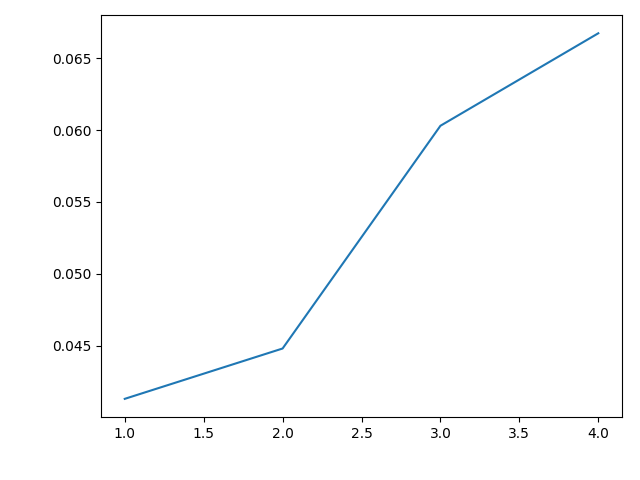
\includegraphics[width=0.8\linewidth]{../weak_scaling.png}
  \caption{Weak scaling plot. A increase in the dimension of the problem
  results in approximately a cubic increase in number of FLOPS, so the
following dimensions were used for 1, 2, 3, and 4 GPUs respectively: 
280, 353, 404, and 445.}
\end{figure}

When evaluating weak scaling, I only scaled the quantity of GPUs. The total
number of CPU threads remained constant. \\

\section{Conclusions}

Communication which has to go through the CPU quickly became the limiting
factor when using multiple GPUs. I would imagine that with effective use of GPU
interconnect, the scaling would be far better. It would likely be possible to
optimize the CUDA kernels by actually fusing the dot product and SpMV
operations in the fused kernel rather than executing them sequentially.
Another potential optimization would be to try half precision. 

\end{document}
